\chapter{GrShell Language}\indexmain{GrShell}
\label{chapgrshell}
\GrShell\ is a \indexedsee{shell}{GrShell} application built on top of \LibGr\indexmain{libGr}.
It belongs to \GrG's standard equipment.
\GrShell\ is capable of creating, manipulating, and dumping graphs as well as performing and debugging graph rewriting.
The \GrShell\ provides a line oriented scripting language.
\GrShell\ scripts are structured by simple statements separated by line breaks.

%rewrite stuff to be command based instead of splitting commands over several sections?


%%%%%%%%%%%%%%%%%%%%%%%%%%%%%%%%%%%%%%%%%%%%%%%%%%%%%%%%%%%%%%%%%%%%%%%%%%%%%%%%%%%%%%%%%%%%%%%%
\section{Building Blocks}

\GrShell\ is \indexed{case sensitive}.
A line may be empty, may contain a shell command, or may contain a comment.
A \indexed{comment} starts with a \indexed{\texttt{\#}} and is terminated by end-of-line or end-of-file.
The following items are required for representing text, numbers, and rule parameters.\\
\\
\emph{Text}\\
May be one of the following:
\begin{itemize}
  \item A non-empty character sequence consisting of letters, digits, and underscores. The first character must not be a digit.
  \item Arbitrary text enclosed by double quotes (\texttt{""}).
  \item Arbitrary text enclosed by single quotes (\texttt{''}).
\end{itemize}
Due to the chosen parser generator shell keywords are not allowed for type names, attribute values and other entities (even if they are legal in the rule language). If this hits you, you can enclose the identifier by single or double quotes, i.e. Text can be used everywhere an identifier is required.

\mbox{ }\\
\emph{Number}\\
Is an \texttt{int} or \texttt{float} constant in decimal notation (see also Section~\ref{sec:builtintypes}).

\begin{rail}
 Parameters : Text + ',' ;
 SpacedParameters: Text + ;
\end{rail}\ixnterm{Parameters}\ixnterm{SpacedParameters}

In order to describe the commands more precisely, the following (semantic) specializations of \emph{Text} are defined:
\begin{description}
  \item[Filename]A fully qualified file name without spaces (e.g.\ \texttt{/Users/Bob/amazing\textunderscore file.txt}) or a single quoted or double quoted fully qualified file name that may contain spaces (\texttt{"/Users/Bob/amazing file.txt"}).
  \item[Variable] Identifier of a (graph global) variable that contains a graph element or a value. \indexmainsee{GrShell variable}{graph global variable} A double colon prefix as required in the sequences may be given, but as the shell only knows graph global variables, it is optional.
  \item[NodeType, EdgeType] Identifier of a node type resp.\ edge type defined in the model of the current graph.
  \item[AttributeName] Identifier of an attribute.
  \item[Graph] Identifies a graph by its name.
  \item[Action] Identifies a rule by its name.
\end{description}
\makeatletter
\begin{rail}
  GraphElement: Text | ('@' '(' Text ')')
\end{rail}\indexmain{\texttt{"@}}\ixnterm{GraphElement}
\makeatother

The elements of a graph (nodes and edges) can be accessed both by their (graph global) \indexed{variable}\indexmain{graph global variable} identifier and by their \newterm{persistent name} specified through a constructor (see Section~\ref{mani}).
The specializations \emph{Node} and \emph{Edge} of \emph{GraphElement} require the corresponding graph element to be a node or an edge respectively.

\begin{example}
\label{persistentex}
We insert a node, \indexed{anonymous}ly and with a \indexed{constructor} (see also Section~\ref{mani}):
\begin{grshell}
> new graph "../lib/lgsp-TuringModel.dll" G
New graph "G" of model "Turing" created.

# insert an anonymous node...
# it will get a persistent pseudo name
> new :State
New node "$0" of type "State" has been created.
> delete node @("$0")

# and now with constructor
> new v:State($=start)
new node "start" of type "State" has been created.
# Now we have a node named "start" and a variable v assigned to "start"
\end{grshell}
\end{example}
\begin{note}
Persistent names will be saved (\texttt{save graph\dots}, see Section~\ref{outputcmds}) and exported,
and, if you visualize a graph (\texttt{dump graph\dots}, see Section~\ref{outputcmds}),
graph elements will be \indexed{label}ed with their persistent names.
Persistent names have to be unique for a graph (the graph they belong to).
\end{note}

\begin{rail}
  Variable '=' ( GraphElement | Variable | Literal )
\end{rail}
Assigns the variable or persistent name \emph{GraphElement} or literal to \emph{Variable}.
If \emph{Variable} has not been defined yet, it will be defined implicitly.
As usual for scripting languages, variables have neither static types nor declarations.
The variables known to \GrShell\ are the graph global variables (see \ref{cha:xgrs} for the distinction between graph global and sequence local variables).

\begin{rail}
'show' 'var' Variable
\end{rail}\ixkeyw{show}\ixkeyw{var}
Prints the content of the specified variable.


%%%%%%%%%%%%%%%%%%%%%%%%%%%%%%%%%%%%%%%%%%%%%%%%%%%%%%%%%%%%%%%%%%%%%%%%%%%%%%%%%%%%%%%%%%%%%%%%
\section{\GrShell\ Commands}
This section describes the \GrShell\ commands\ixnterm{Command}. Commands are assembled from basic elements.
As stated before commands are terminated by line breaks. Alternatively commands can be terminated by the \indexed{\texttt{;;}} symbol.
Like an operating system shell, the \GrShell\ allows you to span a single command over $n$ lines by terminating the first $n-1$ lines with a \indexed{backslash}.
\begin{rail}
  Script: ((Command ('<line break>' | ';;'))+) '<end of file>' ;
\end{rail}\ixnterm{Script}

%-----------------------------------------------------------------------------------------------
\subsection{Common Commands}
\label{commcommands}
\begin{rail}
  'help' (Command)?
\end{rail}\ixkeyw{help}
Displays an information message describing all the supported commands.
A command \texttt{Command} displayed with \texttt{...} has further help available, which can be displayed with \texttt{help Command}.

\begin{rail}
  'quit' | 'exit'
\end{rail}\ixkeyw{quit}\ixkeyw{exit}
Quits \GrShell. If \GrShell\ is opened in debug mode, a currently active graph viewer (such as \yComp) will be closed as well.

\begin{rail}
  'include' Filename ('.gz')?
\end{rail}\ixkeyw{include}
Executes the \GrShell\ script\indexmain{graph rewrite script} \emph{Filename} (which might be zipped).
A \GrShell\ script is just a plain text file containing \GrShell\ commands.
They are treated as they would be entered interactively, except for parser errors.
If a parser error occurs, execution of the script will stop immediately.

\begin{rail}
  'echo' Text
\end{rail}\ixkeyw{echo}
Prints \emph{Text} onto the \GrShell\ command prompt.

\begin{rail}
  'pwd'
\end{rail}\ixkeyw{pwd}
Prints the path to the current working directory.

\begin{rail}
  'ls'
\end{rail}\ixkeyw{ls}
Lists the directories and files in the current working directory, files relevant to GrGen are printed highlighted.

\begin{rail}
  'cd' Path
\end{rail}\ixkeyw{cd}
Changes the current working directory to the path given.

\begin{rail}
  'askfor';
  Variable '=' 'askfor' Type
\end{rail}\ixkeyw{askfor}
The \texttt{askfor} command just waits until the user presses enter.
The \texttt{askfor} assignment interactively asks the user for a value of the specified type.
The entered value is type checked against the expected type, and assigned to the given variable in case it matches.
If the type is a value type, the user is prompted to enter a value literal with the keyboard.
If the type is a graph element type, the user is prompted to enter the graph element by double clicking in yComp.
Note that in this case the debug mode must have been enabled before.
(The command is equivalent to \verb#debug exec Variable=$%(Type)#.)

\begin{example}
\begin{grshelllet}
x = askfor int
\end{grshelllet}
asks the user to enter an integer value; pressing 4 then 2 then enter will do fine.
\begin{grshelllet}
x = askfor Node
\end{grshelllet}
asks the user to select a graph element in yComp; double clicking any node will do fine.
\end{example}

\begin{rail}
  '!' CommandLine
\end{rail}\indexmain{\texttt{"!}}
\emph{CommandLine}\indexmain{command line} is an arbitrary text, the operating system attempts to execute.
\begin{example}
On a Linux machine you might execute
\begin{grshell}
!sh -c "ls | grep stuff"
\end{grshell}
\end{example}

\begin{rail}
'silence' ('on'|'off')
\end{rail}\ixkeyw{silence}\ixkeyw{on}\ixkeyw{off}
Switches the new node / edge created / deleted messages on(default) or off.
Switching them off allows for much faster execution of scripts containing a lot of creation commands.

\begin{rail}
'silence' 'exec' ('on'|'off')
\end{rail}\ixkeyw{silence}\ixkeyw{exec}\ixkeyw{on}\ixkeyw{off}
During non-debug sequence execution every second match statistics are printed to the console;
they allow to assess the progress of long-running transformations.
With this command they can be disabled (or enabled again).
Switching them off may be of interest if own debug messages printed via emit from the sequences (or rules) should not be disturbed.

\begin{rail}
'randomseed' (Number | 'time')
\end{rail}\ixkeyw{randomseed}\ixkeyw{time}
Sets the random seed to the given number for reproducible results when using the \$-operator-prefix or the random-match-selector, whereas time sets the random seed to the current time in ms.

\begin{rail}
'redirect' 'emit' Filename
\end{rail}\ixkeyw{redirect}\ixkeyw{emit}
Redirects the output of the emit-statements in the rules from stdout to the given file.

\begin{rail}
'redirect' 'emit' '-'
\end{rail}\ixkeyw{redirect}\ixkeyw{emit}
Redirects the output of the emit-statements in the rules to stdout (again).

%-----------------------------------------------------------------------------------------------
\subsection{Graph Commands}
\label{graphcommands}

\begin{rail}
  'new' 'graph' Filename Text
\end{rail}\ixkeyw{new}\ixkeyw{graph}
Creates a new graph with the model specified in \emph{Filename}\indexmain{graph model}.
Its name is set to \emph{Text}.
The model file can be either source code (e.g.\ \texttt{turing\textunderscore machineModel.cs}) or a .NET assembly (e.g.\ \texttt{lgsp-turing\textunderscore machineModel.dll}).
It's also possible to specify a rule set file as \emph{Filename}.
In this case the necessary assemblies will be created on the fly.

\begin{rail}
  'new' 'add' 'reference' Filename
\end{rail}\ixkeyw{new}\ixkeyw{add}\ixkeyw{reference}
Configures a reference to an external assembly \emph{Filename} to be linked into the generated assemblies, maps to the \texttt{-r} option of \texttt{grgen.exe} (cf. \ref{grgenoptions}).

\begin{rail}
  'new' 'set' ('keepdebug'|'lazynic'|'noinline') ('on'|'off')
\end{rail}\ixkeyw{new}\ixkeyw{set}\ixkeyw{keepdebug}\ixkeyw{lazynic}\ixkeyw{on}\ixkeyw{off}
Configures the compilation of the generated assemblies to keep the generated files and to add debug symbols,
or configures the generation of the matchers to execute negatives, independents, and conditions only at the end of matching (normally asap),
or configures the generation of the matchers to never inline subpatterns.
Maps to the \texttt{-keep} and the \texttt{-debug} options or to the \texttt{-lazynic} or to the \texttt{-noinline} option of \texttt{grgen.exe} (cf. \ref{grgenoptions}).

\begin{rail}
  'show' 'graphs'
\end{rail}\ixkeyw{show}\ixkeyw{graph}
Displays a list of currently available graphs.

\begin{rail}
  'select' 'graph' Graph
\end{rail}\ixkeyw{select}\ixkeyw{graph}
Selects the current \indexed{working graph}.
This graph acts as \emph{\indexed{host graph}} for graph rewrite sequences (see also Sections~\ref{ov:whatsallabout} and~\ref{grsthings}).
Though you can define multiple graphs, only one graph can be the active ``working graph''.

\begin{rail}
  'clear' 'graph' (() | Graph)
\end{rail}\ixkeyw{clear}\ixkeyw{graph}
Deletes all graph elements of the current working graph resp.\ the graph \emph{Graph}.

\begin{rail}
  'delete' 'graph' Graph
\end{rail}\ixkeyw{delete}\ixkeyw{graph}
Deletes the graph \emph{Graph} from the backend storage.

%-----------------------------------------------------------------------------------------------
\subsection{Validation Commands}

\GrG\ offers two different graph validation mechanisms,
the first checks against the connection assertions specified in the model,
the second checks against an arbitrary graph rewrite sequence containing arbitrary tests and rules.

\begin{rail}
  'validate' ('exitonfailure')? ('strict' ('only' 'specified')?)?
\end{rail}\ixkeyw{validate}\ixkeyw{exitonfailure}\ixkeyw{strict}\ixkeyw{only}\ixkeyw{specified}
Validates\indexmain{validate} if the current working graph fulfills the \indexed{connection assertion}s specified in the corresponding graph model (cf. ~\ref{sct:ConnectionAssertions}).
Validate without the strict modifier checks the multiplicities of the connections it finds in the host graph,
it ignores node-edge-node connections which are available in the host graph but have not been specified in the model.
The \emph{strict} mode additionally requires that all the edges available in the host graph must have been specified in the model.
This requirement is too harsh for models where only certain parts are considered critical enough to be checked
or might be a too big step in tightening the level of structural checking in an already existing large model.
So some form of selective strict checking is supported:
The \emph{strict only specified} mode requires strict matching (i.e. that all edges are covered) only of the edges for which connection assertions have been specified in the model.

\begin{rail}
  'validate' ('exitonfailure')? ('exec'|'xgrs') GRS
\end{rail}\ixkeyw{validate}\ixkeyw{exitonfailure}\ixkeyw{xgrs}\ixkeyw{exec}
Validates\indexmain{validate} if the current working graph satisfies the \indexed{graph rewrite sequence} given.
Before the graph rewrite sequence is executed, the instance graph gets cloned;
the sequence operates on the clone, allowing you to change the graph as you want to, without influence on the host graph.
Validation fails iff the sequence fails.
This gives a rather costly but extremely flexible and powerful mechanism to specify graph constraints.
The GrShell is exited with an error code if \texttt{exitonfailure} is specified and the validation fails.

\begin{example}
We reuse a simplified version of the road map model from Chapter~\ref{chapmodellang}:
\begin{grgen}
model Map;

node class city;
node class metropolis;

edge class street;
edge class highway
      connect metropolis [+] --> metropolis [+];
\end{grgen}
The node constraint on \emph{highway} requires all the metropolises to be connected by highways. Now have a look at the following graph:
\begin{center}
  \fbox{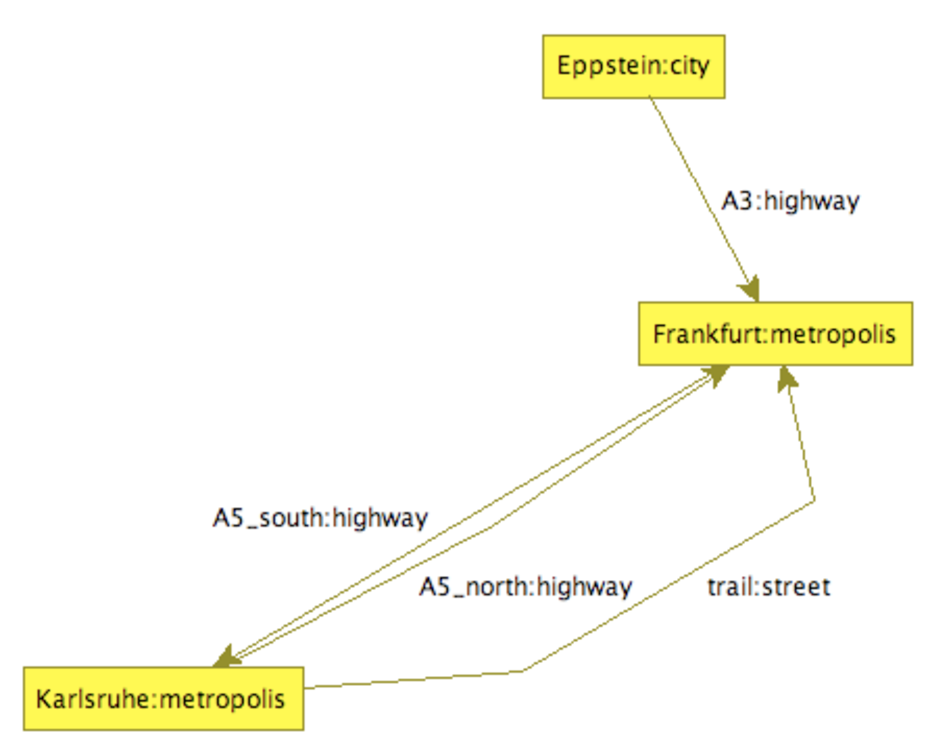
\includegraphics[width=8.5cm]{fig/map}}
\end{center}

This graph is valid but not strict valid.
\begin{grshell}
> validate
The graph is valid.
> validate strict only specified
The graph is NOT valid:
  CAE: city "Eppstein" -- highway "A3" --> metropolis "Frankfurt" not specified
> validate strict
The graph is NOT valid:
  CAE: city "Eppstein" -- highway "A3" --> metropolis "Frankfurt" not specified
  CAE: metropolis "Karlsruhe" -- street "trail" --> metropolis "Frankfurt" not specified
>
\end{grshell}
\end{example}


\pagebreak

%-----------------------------------------------------------------------------------------------
\subsection{Graph Input and Output Commands}
\label{outputcmds}

\begin{rail}
  'save' 'graph' Filename
\end{rail}\ixkeyw{save}\ixkeyw{graph}
Dumps\indexmain{dumping graph} the current graph as \GrShell\ script\indexmain{graph rewrite script} into \emph{Filename}.
The created script includes
\begin{itemize}
  \item selecting the backend
  \item creating a new graph with all nodes and edges (including their persistent names)
  \item restoring the (graph global) variables
  \item restoring the visualisation styles
\end{itemize}
but not necessarily using the same commands you typed in during construction.
Such a script can be loaded and executed by the \texttt{include} command (see Section~\ref{commcommands}).

\begin{rail}
  'export' Filename ('.grs' | '.grsi') ('.gz')?
\end{rail}\ixkeyw{export}\indexmain{export}
Exports an instance graph in GRS (.grs/.grsi) format, which is a reduced \GrShell\ script
(it can get imported and exported on API level\ref{sub:imexport} without using the \GrShell).
This is the recommended standard format.
It contains the \texttt{new graph} command, followed by \texttt{new node} commands, followed by \texttt{new edge} commands.
If the \texttt{.gz} suffix is given the graph is saved zipped.
The export is only complete with the model of the graph given in the \texttt{.gm} file.
Exporting fails if the graph model contains attributes of \texttt{object}-type.
The \texttt{save} command is for saving about a \GrShell\ session including graph global variables and visualization commands,
the goal of the \texttt{export} command is basic graph rewrite system interoperability.

\begin{rail}
  'export' Filename '.gxl' ('.gz')?
\end{rail}\ixkeyw{export}\indexmain{import}
Exports an instance graph and a graph model in GXL format \cite{GXL,GXL2},
which is somewhat of a standard format for graphs of graph rewrite systems,
but suffers from the well-known XML problems -- it is barely human-readable and bloated.
(Besides tools claiming to support it often can't import the export of the other.)
Exporting fails if the graph model contains attributes of \texttt{set<S>}-,\texttt{map<S,T>}-,\texttt{array<S>}- or \texttt{object}-type.
If the \texttt{.gz} suffix is given the graph is saved zipped.

\begin{rail}
  'export' Filename '.grg' ('.gz')?
\end{rail}\ixkeyw{export}\indexmain{import}
Exports an instance graph in GRG format, i.e. as one GrGen rule with an empty pattern and a large modify part.
There is no importer existing, this format is not for normal use!
If the \texttt{.gz} suffix is given the graph is saved zipped.

\pagebreak %force better layout

\begin{rail}
  'import' Filename ('.grs' | '.grsi' ) ('.gz')? (ModelOverride)?
\end{rail}\ixkeyw{import}
Imports the specified graph instance in GRS (.grs/.grsi) format (the \emph{reduced} \GrShell\ script,
a saved graph can only be imported by \texttt{include} (but an exported graph can be imported by \texttt{include}, too)).
The graph model referenced in the .grs/.grsi must be available as \texttt{.gm}-file.
If a model override of the form \texttt{Filename.gm} is specified, the given model will be used instead of the model referenced in the GRS file.
If a model override of the form \texttt{Filename.grg} is specified, the model(s) of the given rule file will be used instead of the model in the GRS file.
If the \texttt{.gz} suffix is given the graph is expected to be zipped.

\begin{rail}
  'import' Filename '.gxl' ('.gz')? (ModelOverride)?
\end{rail}\ixkeyw{import}
Imports the specified graph instance and model in GXL format.
If a model override of the form \texttt{Filename.gm} is specified, the given model will be used instead of the model in the GXL file.
If a model override of the form \texttt{Filename.grg} is specified(s), the model of the given rule file will be used instead of the model in the GXL file.
The \texttt{.gxl}-graph must be compatible to the \texttt{.gm}-model/\texttt{.grg}-model.
If the \texttt{.gz} suffix is given the graph is expected to be zipped.

\begin{note}\label{shellgxlimport}
Normally you are not only interested in importing a GXL graph (and viewing it), but you want to execute actions on it.
The problem is that the actions are model dependent.
So, in order to apply actions, you must use a model override, which works this way:
\begin{enumerate}
\item \texttt{new graph "YourName.grg"}\\
This creates the model library lgsp-YourNameModel.dll
and the actions library lgsp-YourNameActions.dll
(which depends on the model library generated from the \texttt{"using YourName;"}).
\item \texttt{import InstanceGraphOnly.gxl YourName.gm}\\
This imports the instance graph from the .gxl but uses the model specified
in YourName.gm (it must fit to the model in the .gxl in order to work).
\item \texttt{select actions lgsp-YourNameActions.dll}\\
This loads the actions from the actions library in addition to the already
loaded model and instance graph (cf. \ref{grsthings}).
\item Now you are ready to use the actions.
\end{enumerate}
As of version 3.0beta you can specify a \texttt{.grg} as model override;
basically it does what the given enumeration does.
\end{note}

\begin{note}\label{shellecoreexport}
Further formats available for import are \texttt{.ecore} plus \texttt{.xmi} of Eclipse Modeling Framework (EMF).
These are formats common to the model transformation community which are not directly geared towards graphs, so they can't be imported directly.
Instead during the import process an intermediate \texttt{.gm} is written which is equivalent to the \texttt{.ecore} given -- you may inspect it to see how the content gets mapped
(the importer maps classes to GrGen node classes, their attributes
to corresponding GrGen attributes, and their references to GrGen
edge classes; inheritance is transferred one-to-one, and enumerations are
mapped to GrGen enums;
class names are prefixed by the names of the packages they are contained in
and edge type names are prefixed by the names of the node types they originate from,
to prevent name clashes).
After this metamodel transformation the instance graph XMI adhering to the Ecore model thus adhering to the just
generated equivalent GrGen graph model gets imported.
Furthermore you can give specify a \texttt{.grg} containing the rules to apply (using further rule and model files).
An export is not available -- we coded the export we needed for the GraBaTs/TTC challenges the importer was written for with emit statements.
\begin{rail}
  'import' ((Filename '.ecore')+( )) Filename '.xmi' (Filename '.grg')?
\end{rail}\ixkeyw{import}
\end{note}

\begin{rail}
  'import' 'add' FileSpec
\end{rail}\ixkeyw{import}\ixkeyw{add}
Imports the graph in the specified file and adds it to the current graph
(instead of overwriting the old graph with the new graph).
The \texttt{FileSpec} is of the same format as the file specification in the other two imports.

%-----------------------------------------------------------------------------------------------
\subsection{Graph Change Recording and Replaying}
\label{recordnreplay}

\begin{rail}
  'record' Filename ('.gz')? ('start' | 'stop')?
\end{rail}\ixkeyw{record}\ixkeyw{start}\ixkeyw{stop}\indexmain{record}
The record command starts or stops recording of graph changes to the specified file. If neither start nor stop are given, recording to the specified file is toggled (i.e. started if no recording to the file is underway or stopped if the file is already recorded to).
Recording starts with an export (cf. \ref{outputcmds}) of the instance graph in GRS (.grs/.grsi) format, afterwards the command returns but all changes to the instance graph are recorded to the file until the recording stop command is issued.
Furthermore the values given in the \texttt{record} statements (cf. \ref{recstmt}) from the sequences are written to the recording (this allows you to mark states).
If the \texttt{.gz} suffix is given the recording is saved zipped.
You may start and stop recordings to different files at different times, every file receives the graph changes and records statements occuring during the time of the recording.
Note: As a debugging help a recording does not only contain graph manipulation commands (cf. \ref{mani}) but also comments telling about the rewrites and transaction events which occured (whose effects were recorded).

\begin{rail}
  'replay' Filename ('.gz')? ('from' Text)? ('to' Text)?
\end{rail}\ixkeyw{replay}\ixkeyw{from}\ixkeyw{to}\indexmain{replay}
The replay command plays a recording back: the graph at the time the recording was started is recreated, then the changes which occured are carried out again, so you end up with the graph at the time the recording was stopped. Instead of replaying the entire GRS file you may restrict replaying to parts of the file by giving the line to start at and/or the line to stop at. Lines are specified by their textual content which is searched in the file.
If a \emph{from} line is given, all lines from file begin on including this line are skipped, then replay starts. If a \emph{to} line is given, only the lines from the starting point on, until-excluding this one are executed (i.e. all lines from-including this one until file end are skipped).
Normally you reference with \texttt{from} and \texttt{to} comment lines you write with the \texttt{record} statement (cf. \ref{recstmt}) in the sequences, marking relevant states during a transformation process.
An example for record and replay is given in \texttt{tests/recordreplay}.

%-----------------------------------------------------------------------------------------------
\subsection{Graph Manipulation Commands}
\label{mani}
Graph manipulation commands alter existing graphs;
they allow to create, retype and delete graph elements and change attributes.
These are tasks which are or at least should be carried out by the rules of the rule language in the first place.
On shell level they are available and mainly used as elementary instructions in creating an initial graph, in exporting and importing a graph, as well as in change recording and replaying.

\begin{rail}
  'new' (() | Text) (() | ':' NodeType (() | Constructor))
\end{rail}\ixkeyw{new}
Creates a new node within the current graph.
Optionally a variable \emph{Text} is assigned to the new node.
If \emph{NodeType} is supplied, the new node will be of type \emph{NodeType} and attributes can be initialized by a constructor.
Otherwise the node will be of the base node class type \emph{Node}.
\begin{note}
The \GrShell\ can reassign \indexed{variable}s.
This is in contrast to the rule language (Chapter~\ref{chaprulelang}), where we mainly use \emph{names}\indexmain{name}\indexmain{expression variable}\indexmainsee{expression variable}{name}
(with exception of var and ref input variables and def entities).
\end{note}

\begin{rail}
  'new' Node (('-' EdgeEntityConstructor '->') | ('<-' EdgeEntityConstructor '-') | ('-' EdgeEntityConstructor '-')) Node ;
EdgeEntityConstructor:
  (()|Text) (() | ':' EdgeType (() | Constructor)) ;
\end{rail}\ixkeyw{new}
Creates a new edge within the current graph between the specified nodes,
directed from the first to the second \emph{Node} in the case of \texttt{-->},
directed from the second to the first \emph{Node} in the case of \texttt{<--},
or undirected in the case of \texttt{--}.
Optionally a variable \emph{Text} is assigned to the new edge.
If \emph{EdgeType} is supplied, the new edge will be of type \emph{EdgeType} and attributes can be initialized by a constructor.
Otherwise the edge will be of the base edge class type \texttt{Edge} for \texttt{-->} or \texttt{UEdge} for \texttt{--}.

\begin{rail}
  Constructor : '(' (() | (dollar '=' Text (() | ',' Attributes) | Attributes)) ')';
  Attributes : (AttributeName '=' AttributeValue) + (',');
  AttributeValue :  PrimitiveAttributeValue | SetConstr | MapConstr | ArrayConstr;
  PrimitiveAttributeValue : EnumLit | Number | FloatingNumber | QuotedText | BoolLit | NullLit ;
  SetConstr: 'set' '<' Type '>' lbrace ( Expression*',' ) rbrace ;
  MapConstr: 'map' '<' Type ',' Type '>' \\ lbrace ( (Expression '->' Expression)*',' ) rbrace ;
  ArrayConstr: 'array' '<' Type '>' '[' ( Expression*',' ) ']' ;
\end{rail}\indexmain{\texttt{\$}}\ixnterm{Constructor}\ixnterm{Attributes}\ixnterm{AttributeValue}\ixnterm{PrimitiveAttributeValue}\ixnterm{SetConstr}\ixnterm{MapConstr}\ixnterm{ArrayConstr}
A \indexed{constructor} is used to initialize a new graph element (see \texttt{new \dots} below).
A comma separated list of \indexed{attribute} declarations is supplied to the constructor.
Available attribute names are specified by the graph model of the current working graph.
All the undeclared attributes will be initialized with \indexed{default value}s, depending on their type
(\texttt{int} $\leftarrow$ \texttt{0}; \texttt{long} $\leftarrow$ \texttt{0L}; \texttt{byte} $\leftarrow$ \texttt{0Y}; \texttt{short} $\leftarrow$ \texttt{0S}; \texttt{boolean} $\leftarrow$ \texttt{false}; \texttt{float} $\leftarrow$ \texttt{0.0f}; \texttt{double} $\leftarrow$ \texttt{0.0}; \texttt{string} $\leftarrow$ \texttt{""}; \texttt{set<T>} $\leftarrow$ \texttt{set<T>\{\}}; \texttt{map<S,T>} $\leftarrow$ \texttt{map<S,T>\{\}}; \texttt{array<T>} $\leftarrow$ \texttt{array<T>[]}; \texttt{enum} $\leftarrow$ unspecified;).\\
The \texttt{\$} is a special attribute name: a unique identifier of the new graph element.
This identifier is also called \newterm{persistent name} (see Example~\ref{persistentex}).
This name can be specified by a constructor only.

\begin{rail}
  'retype' Node '<' Type '>'
\end{rail}\ixkeyw{retype}
Retypes the node \emph{Node} from its current type to the new type \emph{Type}. Attributes common to initial and final type are kept. Incident edges are kept as well. \indexmain{retype}

\begin{rail}
  'retype' ('-' Edge '<' Type '>' '->' | '-' Edge '<' Type '>' '-')
\end{rail}\ixkeyw{retype}
Retypes the edge \emph{Edge} from its current type to the new type \emph{Type}. Attributes common to initial and final type are kept. Incident nodes are kept as well.

\begin{rail}
  'redirect' Edge ('source'|'target') Node
\end{rail}\ixkeyw{redirect}
Redirects the edge \emph{Edge} from the old source or target node to the new source or target \emph{Node} given.

\begin{rail}
  'delete' 'node' Node
\end{rail}\ixkeyw{delete}\ixkeyw{node}
Deletes the node \emph{Node} from the current graph.
Incident edges will be deleted as well.

\begin{rail}
  'delete' 'edge' Edge
\end{rail}\ixkeyw{delete}\ixkeyw{edge}
Deletes the edge \emph{Edge} from the current graph.

\begin{rail}
  GraphElement '.' AttributeName '=' AttributeValue ;
\end{rail}
Set the \indexed{attribute} \emph{AttributeName} of the graph element \emph{GraphElement} to the value \emph{AttributeValue} (for the different possible attribute values see above).

\begin{rail}
  GraphElement '.' AttributeName '[' Index ']' '=' AttributeValue ;
\end{rail}
Overwrite the value in the array \indexed{attribute} \emph{AttributeName} of the graph element \emph{GraphElement} at the integer position \emph{Index} with the value \emph{AttributeValue}.

\begin{rail}
  GraphElement '.' AttributeName '.' 'add' '(' \\
  	PrimitiveAttributeValue (',' PrimitiveAttributeValue)? ')' ;
\end{rail}
Add the value \emph{PrimitiveAttributeValue} (for the different possible primitive attribute values see above) to the set valued attribute \emph{AttributeName} of the graph element \emph{GraphElement} or add the key-value pair consisting of the two \emph{PrimitiveAttributeValue}s to the map valued attribute \emph{AttributeName} of the graph element \emph{GraphElement}.
Or add the value \emph{PrimitiveAttributeValue} to the end of the array valued attribute \emph{AttributeName} of the graph element \emph{GraphElement} in the one parameter case or insert the \emph{PrimitiveAttributeValue} to the of the array valued attribute \emph{AttributeName} of the graph element \emph{GraphElement} at the index given by the second parameter in the two parameter case.

\begin{rail}
  GraphElement '.' AttributeName '.' 'rem' '(' (PrimitiveAttributeValue)? ')' ;
\end{rail}
Remove the value \emph{PrimitiveAttributeValue} from the set valued attribute \emph{AttributeName} of the graph element \emph{GraphElement} or remove the key \emph{PrimitiveAttributeValue} from the map valued attribute \emph{AttributeName} of the graph element \emph{GraphElement} or remove the index \emph{PrimitiveAttributeValue} from the array valued attribute \emph{AttributeName} of the graph element \emph{GraphElement} or remove the end element from the array valued attribute \emph{AttributeName} of the graph element \emph{GraphElement} in the zero parameter case.

%-----------------------------------------------------------------------------------------------
\subsection{Graph and Model Query Commands}

\begin{rail}
  'show' (() | 'num') ('nodes' (() | (() | 'only') NodeType) | 'edges' (() | (() | 'only') EdgeType))
\end{rail}\ixkeyw{show}\ixkeyw{num}\ixkeyw{nodes}\ixkeyw{edges}\ixkeyw{only}
Gets the \indexed{persistent name}s and the types of all the nodes/edges of the current graph.
If a node type or edge type is supplied, only elements compatible to this type are considered.
The \texttt{only} keyword excludes subtypes. Nodes/edges without persistent names are shown with a pseudo-name.
If the command is specified with \texttt{num}, only the number of nodes/edges will be displayed.

\begin{rail}
  'show' ('node' | 'edge') 'types'
\end{rail}\ixkeyw{show}\ixkeyw{node}\ixkeyw{edge}\ixkeyw{types}
Gets the node/edge types of the current graph model.

\begin{rail}
'show' ('node' ('super' | 'sub') 'types' NodeType | 'edge' ('super' | 'sub') 'types' EdgeType)
\end{rail}\ixkeyw{show}\ixkeyw{node}\ixkeyw{edge}\ixkeyw{super}\ixkeyw{sub}\ixkeyw{types}\indexmain{inheritance}
Gets the inherited/descendant types of \emph{NodeType}/\emph{EdgeType}.

\begin{rail}
  'show' ('node' 'attributes' (() | (() | 'only') NodeType) | 'edge' 'attributes' (() | (() | 'only') EdgeType))
\end{rail}\ixkeyw{show}\ixkeyw{node}\ixkeyw{edge}\ixkeyw{only}\ixkeyw{attributes}
Gets the available node/edge \indexed{attribute} types.
If \emph{NodeType}/\emph{EdgeType} is supplied, only attributes defined in \emph{NodeType}/\emph{EdgeType} are diplayed.
The \texttt{only} keyword excludes inherited attributes.\\
\begin{warning}
The \texttt{show nodes/edges attributes\dots} command covers types and \emph{inherited} types.
This is in contrast to the other \texttt{show\dots} commands where types and \emph{sub}types are specified or the direction in the type hierarchy is specified explicitly, respectively.
\end{warning}

\begin{rail}
 'show' ('node' Node | 'edge' Edge)
\end{rail}\ixkeyw{show}\ixkeyw{node}\ixkeyw{edge}
Gets the attribute types and values of a specific graph element.

\begin{rail}
  'show' GraphElement '.' AttributeName
\end{rail}\ixkeyw{show}
Displays the value of the specified attribute.

\begin{rail}
  'node' 'type' Node 'is' Node | 'edge' 'type' Edge 'is' Edge
\end{rail}\ixkeyw{node}\ixkeyw{edge}\ixkeyw{type}\ixkeyw{is}
Gets the information whether the first element is \indexed{type-compatible}\indexmainsee{compatible types}{type-compatible} to the second element.


%-----------------------------------------------------------------------------------------------
\subsection{Action Commands (XGRS)}\indexmain{action command}\indexmainsee{action}{graph rewrite sequence}
\label{grsthings}
An \emph{action} denotes a graph rewrite rule.

\begin{rail}
  'select' 'actions' Filename
\end{rail}\ixkeyw{select}\ixkeyw{actions}
Selects a \indexed{rule set}.
\emph{Filename} can either be a .NET assembly (e.g.\ ``rules.dll'') or a source file (``rules.cs'').
Only one rule set can be loaded simultaneously.

\begin{rail}
  'show' 'actions'
\end{rail}\ixkeyw{show}\ixkeyw{actions}
Lists all the rules of the loaded rule set, their parameters, and their return values.
Rules can return a set of graph elements.

\begin{rail}
  'custom' 'actions' (() | SpacedParameters)
\end{rail}\ixkeyw{custom}\ixkeyw{actions}
Executes an action specific to the current \indexed{backend}.
If \emph{SpacedParameters} is omitted, a list of available commands will be displayed (for the LGSPBackend see Section~\ref{custom}).

\begin{rail}
  GraphRewriteSequence: RewriteSequenceDefinition;
\end{rail}\ixkeyw{def}\indexmain{graph rewrite sequence definition}\indexmain{sequence definition}
This command allows to define a named sequence at runtime, for $RewriteSequenceDefinition$ have a look here  \ref{sec:sequencedefinition} in the rule application control language chapter.
Especially it allows to replace an old sequence definition, but only if the signature is identical.
Compiled sequences defined in rule files can't be replaced.
The defined sequence can then be used from following graph rewrite sequences (or following sequence definitions) in the shell.

\begin{example}
\begin{grgen}
# a sequence definition (of an interpreted sequence) is only available
# after it was registered the first time
# but it can get overwritten with a sequence of the same signature
# -> (self or mutually) recursive sequences must be constructed with empty body first
def chain(first:A):(last:A){ true }
def chain(first:A):(last:A){ if{(next:A)=chainPiece(first); (last)=chain(next); last=first} }
\end{grgen}
\end{example}

\makeatletter
\begin{rail}
  GraphRewriteSequence: ('exec'|'xgrs') SimpleRewriteSequence ;
\end{rail}\ixkeyw{exec}\ixkeyw{xgrs}\indexmain{graph rewrite sequence}\indexmainsee{GRS}{graph rewrite sequence}\ixnterm{GraphRewriteSequence}
This executes the graph rewrite sequence \emph{SimpleRewriteSequence}.
See Chapter~\ref{cha:xgrs} for graph rewrite sequences.
Additionally to the variable assignment in rule-embedded graph rewrite sequences, you are also able to assign \emph{persistent names} to parameters via  \texttt{Variable = \@(Text)}.

Graph elements returned by rules can be assigned to variables\indexmain{variable} using \texttt{(Para\-meters) = \emph{Action}}\indexmain{parameter}.
The desired variable identifiers have to be listed in \emph{Parameters}.
Graph elements required by rules must be provided using \texttt{Action (Para\-meters)}, where \emph{Parameters} is a list of variable identifiers.
For \indexed{undefined variables} see Section~\ref{ruledecls}, \emph{Parameters}.


%%%%%%%%%%%%%%%%%%%%%%%%%%%%%%%%%%%%%%%%%%%%%%%%%%%%%%%%%%%%%%%%%%%%%%%%%%%%%%%%%%%%%%%%%%%%%%%%
\section{Backend Commands}
\label{backend}

\GrG\ is built to support multiple backends implementing the model and action interfaces of libGr.
This is roughly comparable to the different storage engines MySQL offers.
Currently only one backend is available, the libGr search plan backend, or short LGSPBackend.

\subsection{Backend Selection and Custom Commands}

\begin{rail}
  'select' 'backend' Filename ( ( ) | ':' Parameters )
\end{rail}\ixkeyw{select}\ixkeyw{backend}
Selects a \indexed{backend} that handles graph and rule representation.
\emph{Filename} has to be a .NET assembly (e.g.\ \texttt{lgspBackend.dll}\indexmain{LGSPBackend}).
Comma-separated \indexed{parameter}s can be supplied optionally; if so, the backend must support these parameters.
By default the LGSPBackend is used.

\begin{rail}
  'show' 'backend'
\end{rail}\nopagebreak\ixkeyw{show}\ixkeyw{backend}
List all the parameters supported by the currently selected backend.
The parameters can be provided to the \texttt{select backend} command.

\begin{rail}
  'custom' 'graph' ( ( ) | SpacedParameters )
\end{rail}\ixkeyw{custom}\ixkeyw{graph}
Executes a command specific to the current backend.
If \emph{SpacedParameters} is omitted, a list of available commands will be displayed (for the LGSP backend see Sections~\ref{custom}).


\subsection{LGSPBackend Custom Commands}
\label{custom}

%several rail nts are defines resolved to terminal with underscores

The \indexed{LGSPBackend} supports the following custom commands:

\begin{rail}
  'custom' 'graph' 'analyze'
\end{rail}\ixkeyw{custom}\ixkeyw{graph}\ixkeyw{analyze}
Analyzes\indexmain{analyzing graph} the current working graph.
The analysis data provides vital information for efficient \indexed{search plan}s.
Analysis data is available as long as \GrShell\ is running, i.e.\ when the host graph changes, the analysis data is still available but maybe obsolete.

\begin{rail}
  'custom' 'graph' setmaxmatches Number
\end{rail}\ixkeyw{custom}\ixkeyw{graph}\ixkeyw{setmaxmatches}
Sets the maximum amount of possible pattern matches to \emph{Number}.
This command affects the expression \texttt{[\emph{Rule}]}.
If \emph{Number} is less or equal to zero, the constraint is reset.

\begin{rail}
  'custom' 'graph' 'optimizereuse' BoolLit
\end{rail}\ixkeyw{custom}\ixkeyw{graph}\ixkeyw{optimizereuse}
If set to false it prevents deleted elements from getting reused in a rewrite (i.e. it disables a performance optimization).
If set to true, new elements may not be discriminable anymore from already deleted elements using object equality, hash maps, etc.

\begin{rail}
  'custom' 'actions' gensearchplan (Action*)
\end{rail}\ixkeyw{custom}\ixkeyw{actions}\ixkeyw{gensearchplan}
Creates a search plan (and executable code from it) for each rewrite rule \emph{Action} using the data from analyzing the graph (\texttt{custom graph analyze}).
Otherwise a \indexed{default search plan} is used.
If no rewrite rule is specified, all rewrite rules are compiled anew.
Analyzing and search plan/code generation themselves take some time, but they can lead to (massively) faster pattern matching, thus overall execution times;
the less uniform the type distribution and edge wiring between the nodes, the higher the improvements.
During the analysis phase the host graph must be in a shape ``similar'' to its shape when the main amount of work is done
(there may be some trial-and-error steps at different time points needed to get the overall most efficient search plan.)
A search plan is available as long as the current rule set remains loaded.
Specify multiple rewrite rules instead of using multiple commands for each rule to improve the search plan generation performance.

\begin{rail}
  'custom' 'actions' 'explain' Action
\end{rail}\ixkeyw{custom}\ixkeyw{actions}\ixkeyw{explain}
Shows the search plan currently in use for \emph{Action}, plus the subpatterns called by it.
This is an inspection tool comparable to the \texttt{explain} command offered by SQL-databases to inspect the search plans of their queries.
The explain command allows to evaluate the effects of performance optimization, esp. it allows to change the graph which serves as analysis data source for matcher regeneration, or to annotate the static rules with priorities (cf. \ref{annotations}), until a good search plan is built.
The search plan is shown as a list of search commands (with commands not doing real matching work shown in parenthesis), which is executed from top to bottom; for more on the search commands have a look at section \ref{searchplanning}.

\begin{rail}
  'custom' 'actions' dumpsourcecode BoolLit
\end{rail}\ixkeyw{custom}\ixkeyw{actions}\ixkeyw{dumpsourcecode}
If set to true, C\# files will be dumped for the newly generated searchplans (similar to the \texttt{-keep} option of the generator).


% todo: beispielshellscripte